\rcsInfo $Id: verification.tex,v 1.45 2003/12/04 15:03:06 brucker Exp $

\chapter{Verifying the Consistency and the Refinement}\label{chap:verification}

\section{Consistency Conditions}\label{sec:consistency}

Two types of consistency conditions that we expect in general in a
specification, can be listed:
\begin{enumerate}
\item Logical consistency. This comprises:
  \begin{enumerate}
  \item The \emph{conservativity} of all axiomatic definitions, and
  \item the \emph{definedness} of all relational applications $f(x)$.
  \end{enumerate}
\item Methodological consistency. This comprises the $deadlock$-$freeness$ of
  all operations.
\end{enumerate}

Conservativity can be assured if it is syntactically checked that all axiomatic
definitions belong to one of the following \emph{conservative axiom schemes}
described by~\cite{gordon.ea:hol:1993}, which also form the basis of the
Isabelle/HOL libraries.  Here, we briefly review the five most essential
schemes:
\begin{enumerate}
\item The \emph{constant definition}: An equational, non-recursive axiom
  introducing a fresh constant as an ``abbreviation'' of already defined
  concepts.
\item The \emph{constant specification}: An arbitrary predicate $P(c)$ over a fresh
  constant $c$; as proof obligation, it remains to show that there is a witness of
  the predicate: $\exists x. P(x)$.
\item The \emph{type definition}: A fresh type constructor is defined via an
  isomorphism to a set of values defined before.
\item The \emph{well-founded recursion} scheme: A recursive axiom for a fresh
  constant that requires that it is applied to ``less'' arguments in all
  occurrences on the right hand side, where ``less'' is understood in terms of a
  preconceived well-founded ordering.
\item The \emph{primitive recursion} scheme: This is a special case of the
  previous definition scheme.
\end{enumerate}

Note that the latter two schemes were mapped to constant definitions in
Isabelle/HOL; the necessary proof work is performed by the system behind the scene.
Unfortunately, currently HOL-Z does not automatically check the side-conditions
of conservativity according to these schemes (as, in contrast, Isabelle/HOL
does).  Hence, throughout this paper, these checks have been established by
reviews --- a mechanical check for these conditions, although highly desirable 
since specifications are constantly changed during development,
has not been implemented so far. 

The second type of logical inconsistency condition is not crucial from a HOL
point of view; relational application is defined by the Hilbert operator:
\begin{lstlisting}{}
   f(x) == @ y. (x,y) : f
\end{lstlisting}
such that from the HOL point-of-view, these expressions are well-defined -- but
arbitrary. With respect to Z semantics, this kind of expression is $undefined$.
This means that Z is semantically more restrictive, and these situations should
be avoided.  Thus, in the case of HOL-Z, this boils down to the proof that for
all relational applications $f(x)$, $x$ actually belongs to the declared domain
of $f$.

Methodological consistency is unproblematic from the logical point of view ---
methodologically inconsistent operations are just non-left-total relations ---,
but from the pragmatical point of view, specifications of operations that
represent a deadlock are simply ``wrong'' in the sense that they do not model
real operational behavior. Therefore, checks of this kind help to find errors
in the specification. Here, ``deadlock-freeness'' of an operation means that for
any \emph{legal} input $x?$ and a given $state$, there must be at least one
possible output $y!$ (if output parameters were defined) and a successor state
$state'$. In other words, whenever an operation is given legal input in a
consistent state, a transition to a consistent successor state is assured. This
condition can be compactly represented by the schema operator $pre op$ for any
given schema $op$, which is equivalent to $\exists y! state'. op$.  The question
remains to settle what ``legal'' input $x?$ is. As such, we consider input that
fulfills all constraints in the body of a schema, more precisely, all these
conjoints in the body, that contain only occurrences of input variables (i.e.\
variables with a $?$-suffix) or state variables (i.e.\  variables that do not
have a stroke-suffix or an exclamation mark suffix). We call the conjunction of
all conjoints fulfilling this condition the \emph{syntactic precondition}
$syn\_pre$ of an operation schema $op$. On this basis, we can define
deadlock-freeness schematically as:
\[
   df_{op} \equiv syn\_pre_{op} \implies pre op
\]
In a backward proof, a theorem of deadlock-freeness can be used to reduce the
proof-task $pre op$ just to the syntactic precondition. It turns out that this
step is crucial for proving the first refinement condition (see
Section~\ref{sec:refinement}). Therefore, theorems of deadlock-freeness 

\subsection{The Conservativity of the System Architecture}
First, recall that all schema definitions and all schema logical definitions are
non-recursive definitions as ``sets of records'', thus constant
definitions. Therefore, only axiomatic definitions remain to consider.
Manually, it is easy to check that only non-polymorphic constant definitions are
used throughout all axiomatic definitions. There are two exceptions:
\begin{enumerate}
\item The specification of $cvs\_perm\_order$ in Section~\ref{sec:basics},
      which is in fact a constant specification: recall that 
      $cvs\_perm\_order$ must be a partial order (reflexive, transitive,
      antisymmetric) with $cvs\_public$ as least and $cvs\_admin$ as greatest
      elements. Such an ordering exists; witness for it is just the trivial
      ordering $\{(cvs\_public,cvs\_admin)\}$.
\item The operation $cutPath$ is a relict due to laziness: it can be
  reformulated as constant definition easily via the Hilbert-Operator.
\end{enumerate}

\subsection{The Definedness of the System Architecture}
In the following, we will list the definedness conditions.
The proofs (mostly done by H. Hiss in his ``Studienarbeit'' are contained
in special \verb+.ML+-files contained in the HOL-Z distribution (see
\verb+examples/zeta/cvs-server/holz+). The proofs are in their vast majority
just calls of Isabelle's \verb+auto+-tactics.
%
%HH adds:
%

In general, the question $(x \in \dom f)$ is not decidable. In the CVS server
specification, approximately 50 percent of the functions are total functions.
Total functions are a special case which makes the task of proving the
obligations easier, as Z specifications require all variables to be declared on
sets which are usually equal to the domain of the function. The proof is
simplified to finding the set constraint declaration of the variable (e.g.\ via
expanding schemas) and using the function declaration as main argument for an
automatic proof. The remaining proofs have to be considered individually.
Provided that the goal is provable, after inserting few implication steps using
facts and predicates from the specification, they can be handled in a fast and
simple manner.

For formulating all definedness consistency conditions, it was necessary to
distinguish whether the function applications appear inside Z-schemas or
axiomatic definitions. Since schemas themselves may be used as predicates, the
definedness goals caused by terms located in schemas can easily be stated within
the schema calculus using schema quantification. In contrast to that,
definedness goals evoked by function applications inside axiomatic definition
environments have to be treated separately, as boolean constants only exist
inside schema predicate parts. The corresponding Isabelle proofs differ only in a few lines. \\
As an example, we perform the procedure for the operation $mkdir$ of the
Z-Section $FileSystem$. The function
application $attributes(wdir)$ produces the condition $mkdir\_cc1$.\\
%
\zcomment{%
    \begin{schema}{mkdir}
    \Delta FileSystem \\
    \Xi ProcessState \\
    u? : Name \\
    \where
    wdir \isdirin files \\
    \lnot ( wdir\cat\langle u? \rangle \isdirin files) \\
    has\_w\_access(uid,wdir,attributes) \\
% otherwise Stale NFS handle: (and on a local drive, e.g.  non-NFS ;-))
%  wdir \in \dom files \\
    
    files' = files \cup \{ wdir \cat \langle u? \rangle \mapsto Inr(Nil) \} \\

    attributes' = ( \< \LET pms  == \{ru,wu,xu,rg,wg,xg,ro,wo,xo\} \setminus
    umask @ \\ 
    \LET pms' == \< \IF sg \in (\fbox{\color{red}attributes(wdir)}).perm   \\
    \THEN pms \cup ((attributes(wdir)).perm \cap \{rg,wg,xg\}) \\
    \ELSE pms @ \>
    \LET wdir\_gid == \< \IF sg \in (attributes(wdir)).perm\\
    \THEN (attributes(wdir)).gid\\
    \ELSE gid @ \> 
    \t1 attributes \oplus \{wdir\cat\langle u?\rangle\mapsto \\
    \t2 \lblot perm==pms',uid==uid,gid==wdir\_gid \rblot \})\>
  \end{schema}}

%
%
Our formulation of the condition $mkdir\_cc1$ uses the Z specific schema
calculus.\\

 \zcomment{\begin{zed} mkdir\_cc1
    == \forall mkdir @ \\
    [ \Delta FileSystem; \Xi ProcessState; u? : Name | wdir \in \dom attributes ]
    \\
\end{zed}} 

The schema all-quantification of $mkdir$ provides the local schema context. It can be used to trivially dissolve the set constraints caused by the signature of the ad-hoc schema\\[0.3cm]
$[ \Delta FileSystem; \Xi ProcessState; u? : Name | wdir \in \dom attributes ]$.\\[0.3cm]
Therefore the definedness consistency condition $mkdir\_cc1$ is made up of the
predicate $(wdir \in \dom attributes)$, with respect to the local context. The
function $attributes$ is an element of the set $FILEATTR\_TAB$ which contains
partial functions ($FILEATTR\_TAB == Path \pfun FILEATTRIBUTES$). This means
that the proof has to be customized and can not immediately be handled like the
proofs for total functions. We first show a paper and pencil proof of
$mkdir\_cc1$ and afterwards illustrate the computer supported proof of it.

\begin{enumerate}
%
% 1. 
%
\item Within the predicate part of the schema $FileSystem$ the following
  equation can be found:
\[
\dom files = \dom attributes
\]
%
% 2.\verb|_isdirin__axdef|
%
\item Inside the axiomatic definition of $isdirin$ and related predicates, there
  is also a formula for the predicate $\isin$:
\begin{center}
$\forall fs : (Path \pfun (Data \pplus Unit)); f:Path @$\\%
$\t1 (f \isin fs) \iff f \in \dom fs$\\
\end{center}
%
% 3.\verb|_isdirin__axdef|
%
\item In the same axiomatic definition, we can find a formula for the
  predicate $\isdirin$:
\begin{center}
$\forall fs: (Path \pfun (Data \pplus Unit)); d: Path @$ \\%
$\t1 (d \isdirin fs) \iff (d \isin fs) \land (\exists u: Unit @ fs(d) = Inr(u))$\\
%$\forall fs : (Path \pfun (Data \pplus \power Name)) ; d:Path@$\\%
%$\t1 (d \isdirin fs) \iff (d \isin fs) \land (\exists m : \power Name @ fs(d) = Inr(m))$\\
\end{center}
%
% 4. 
%
\item Using the definition of $FILESYS\_TAB$ and the declaration of
  $files$ in the schema $FileSystem$, we get:
\begin{center}
$files : FILESYS\_TAB$\\
$FILESYS\_TAB == Path \pfun (Data \pplus Unit)$ \\
$files : Path \pfun (Data \pplus Unit)$
\end{center}
%
% 5. 
%
\item The schema ProcessState contains the following constraint:
\begin{center}
$wdir : Path$\\
\end{center}
%
% 6. 
%
\item In the predicate part of the $mkdir$--operation we can find the
  following prerequisite:
\begin{center}
$wdir \isdirin files$
\end{center}
\end{enumerate}

With these constituents, we can conclude:

\begin{center}
$(6.) wdir \isdirin files \stackrel{(3., 4., 5.)}{\implies} %
wdir \isin files \stackrel{(2.,4.,5.)}{\implies}$\\ %
$wdir \in \dom files \stackrel{(1.)}{\implies} %
wdir \in \dom attributes$
\end{center}
%
To consolidate this proof, here follows a more detailed view in
natural deduction style also showing all basic rules used.\\[0.4cm]
%
%
%
%===================================
%
% the rules which I used in the proof
%
%===================================
\fbox{%
\begin{minipage}{0.97\textwidth}%
  \begin{center}
  %\[
  \begin{prooftree}
    \quad
    \begin{prooftree}
      [A]
      \proofdotseparation=1.2ex
      \proofdotnumber=4
      \leadsto%
      B
    \end{prooftree}
    \justifies
    A \implies B
    \thickness=0.08em
    %\shiftright 0.5cm
    \using
    \mbox{(ImpI)}
    \end{prooftree}%
    \quad\quad\quad\quad%
    \begin{prooftree}
      A \land B
      \justifies
      A
      \using
      \mbox{(AndEl)}
    \end{prooftree}
    \quad\quad\quad\quad%
    \begin{prooftree}
      A\implies B
      \quad A
      \justifies
      B
      %\shiftright 0.5cm
      \using
      \mbox{(Mp)}
    \end{prooftree}
    %\]
  \end{center}
%
    \begin{center}
    %\[%
    \begin{prooftree}
      s=t
      \quad P(s)
      \justifies
      P(t)
      \using
      \mbox{(Subst)}
    \end{prooftree}
    \quad\quad\quad\quad%
    \begin{prooftree}
      y : A
      \quad \forall x : A @ P(x)
      \justifies
      P(y)
      \using
      \mbox{(Bspec)}
    \end{prooftree}
  %  \] 
  \end{center}   
  \end{minipage}%
%
%
}
%-------------------------
%
\begin{center}
  \begin{minipage}{6 cm}
    \vspace{3 mm}
    {A few basic rules}\vspace{3 mm}
  \end{minipage}
\end{center}%
%%
%%===================================
%%
%% small lemma : HS3
%%
%%===================================
%%vorher:\boxed nur
\noindent\fbox{%
  \begin{minipage}{0.97\textwidth}%
    \begin{center}%
    \begin{prooftree}
      \[
        \[
          (A \implies B \land C)
          \quad [A]_1
          \justifies
          B \land C
          \using
          \mbox{(Mp)}
        \]
        \justifies
        B
        \using
        \mbox{(AndEl)}
      \]
      \justifies
      (A \implies B)
      \using
      \mbox{(ImpI)}_1
    \end{prooftree}
    \quad\quad%
    \begin{prooftree}
      (A \implies B \land C)
      \justifies
      (A \implies B)
      \using
      \mbox{(L3)}
    \end{prooftree}
    \end{center}%
  \end{minipage}%
  }\\%
%%-------------------------
%%
\begin{center}
  \begin{minipage}{6 cm}
    \vspace{3 mm}
    {Proof of lemma 3.}\vspace{3 mm}
  \end{minipage}
\end{center}%
%%
%%
%%
%%
%%===============================================
%%
%% Hauptbeweis und Hilfssaetze 1 und 2.
%%
%%===============================================
%%
\begin{landscape}%
\begin{figure}%
\begin{center}%
\begin{prooftree}
  \[
  \mbox{(1.)}
  \justifies
  \begin{array}{l}\dom files \\=\dom attributes\end{array}
  \]
  \quad 
  \[
   \[
   \mbox{lemma 1}
   \justifies
   \begin{array}{l}(wdir \isin files\\ \implies wdir \in \dom files)\end{array}
   \]
   \quad
   \[
     \[
      \[
      \mbox{lemma 2}
      \justifies
      \begin{array}{l}(wdir \isdirin files \\ \implies wdir \isin files \land ?a)\end{array}
      \]
     \justifies
     \begin{array}{l}(wdir \isdirin files \\ \implies wdir \isin files)\end{array}
     \using
     \mbox{(L3)}
     \]
     \quad
     \[
     \mbox{(6.)}
     \justifies
     (wdir \isdirin files)
     \]
   \justifies
   (wdir \isin files)
   \using
   \mbox{(Mp)}
   \]
  \justifies
  wdir \in \dom files
  \using
  \mbox{(Mp)}
  \]
  \justifies
  wdir \in \dom attributes
  \using
  \mbox{(Subst)}
\end{prooftree}
    \end{center}%
\begin{center}%
Proof of $mkdir\_cc1$.%
\end{center}%
\begin{center}%
\begin{prooftree}
    \[
      \[
      (5.)
      \justifies
      wdir : Path
      \]
      \quad
      \[
        \[
        (4.)
        \justifies
        files : FILESYS\_TAB
        \]
        \quad
        \[
        (2.)
        \justifies
        \begin{array}{l}\forall fs : FILESYS\_TAB; d : Path@ \\(d \isin fs \iff d \in \dom fs)\end{array}
        \]
      \justifies
      \forall d : Path@ (d \isin files \iff d \in \dom files)
      \using
      \mbox{(Bspec)}
      \]
    \justifies
    (wdir \isin files \iff wdir \in \dom files)
    \using
    \mbox{(Bspec)}
    \]
  \justifies
  (wdir \isin files \implies wdir \in \dom files)
  \using
  \mbox{(AndEl)}
  \end{prooftree}
\end{center}%
\begin{center}%
Proof of lemma 1.%
\end{center}%
\begin{center}%
\begin{prooftree}
    \[
      \[
      (5.)
      \justifies
      wdir : Path
      \]
      \quad
      \[
        \[
        (4.)
        \justifies
        files : FILESYS\_TAB
        \]
        \quad
        \[
        (3.)
        \justifies
         \begin{array}{l}\forall fs : FILESYS\_TAB; d : Path@ (d \isdirin fs \iff \\(d \isin fs \land (\exists u : Unit @ fs(d) = Inr(u))))\end{array}
        \]
      \justifies
      \forall d : Path@ (d \isdirin files \iff (d \isin files \land a?))
      \using
      \mbox{(Bspec)}
      \]
    \justifies
    (wdir \isdirin files \iff (wdir \isin files \land a?))
    \using
    \mbox{(Bspec)}
    \]
  \justifies
  (wdir \isdirin files \implies (wdir \isin files \land a?))
  \using
  \mbox{(AndEl)}
\end{prooftree}
\end{center}%
\begin{center}%
Proof of lemma 2.%
\end{center}%
%
\caption{Proof of $mkdir\_cc1$ and 2 lemmas.}%
\end{figure}%
\end{landscape}%
%
%
 \begin{figure}
 \begin{center}

   \rotatebox{0}{\scalebox{0.8}{\includegraphics[]{pics/mkdir_cc1.pdf}}}
 %\epsfig{file=mkdir_cc1.ps,height=5.cm}
 \end{center}
 \caption{This is the lemmagraph for the manual proof of $mkdir\_cc1$. The basic rules are inside boxes, and both assumptions and facts found in the specification are printed as numbers.}
 \end{figure}
%
% 
% machine supported proof
%
The machine supported proof of $mkdir\_cc1$ using Isabelle98/HOL-Z can be grouped into five steps.

\begin{enumerate}
\item We formulated the proof obligations in Z. In doing so, the \Zeta~tool
  ensured usage of correct Z syntax and exported both the specification and the
  obligations to a valid HOL-Z format.
%
%
  \begin{center}
\begin{minipage}{.9\linewidth }
\ensuremath{mkdir\_cc}
\zcomment{\begin{zed}
mkdir\_cc1
== \forall mkdir @ \\
[
\Delta FileSystem; \Xi ProcessState; u? : Name | wdir \in \dom attributes
] 
\\
\end{zed}}
\end{minipage}
\end{center}
The HOL-Z \LaTeX\ style automatically generates a nice output of this condition. The following lines result from exporting it to Isabelle.
%
\begin{holzverb}
"mkdir_cc1 ==

      %A mkdir @ +..
                   %Delta SNAME FileSystem (attributes, files);
                   %Xi SNAME ProcessState (gid, uid, umask, wdir); 
                   u? setDecl Name
                 |--
                   wdir : dom attributes
                 -.." 
\end{holzverb}
%
Using this definition, we can start the Isabelle/HOL-Z proof:
\begin{holzverb}
zgoalw SysArchConsistency.thy [mkdir_cc1_def] "mkdir_cc1";
\end{holzverb}
For finding all function applications throughout the whole specification, we
used an ML function which prints each of them grouped by the Z structures where
they appear (zsection, axiomatic definition, schema definition, \dots)
\item In Isabelle/HOL-Z, we start with simplifying the goal by stripping off
  schema quantors and turnstyles and so on~(using \verb|stripS_tac|) and then
  continue by eliminating trivial set constraints which may be found in the
  assumptions either directly or via using a few minor rewrite steps (e.g.\
  expanding schemas).
\item At this point only showing $wdir \in \dom attributes$ is left to us. Using
  one substitution step and the fact $\dom files = \dom attributes$ from the
  predicate part of the $FileSystem$ schema, we reduce this to $wdir \in \dom
  files$.
\begin{holzverb}
by(res_inst_tac [("s","dom files"),("t","dom attributes")] subst 1);
\end{holzverb}
\item Reuse of outsourced lemmas allows us to achieve a higher degree of
  abstraction. The lemma $in\_dom\_if\_isdirin$ can be found in the library
  \verb|FileSystem.ML|.
%
%
\begin{holzverb}
 in_dom_if_isdirin
 =
   "[| ?f : Path -|-> Data + Unit; ?p : Path; (?p, ?f) : _isdirin_ |]
      ==> ?p : dom ?f"  
\end{holzverb}
%
\item The remaining subgoals can be erased trivially either directly or
  indirectly similarly as mentioned in step 2. One could envisage an ML function
  which tries solving a given goal by recursively expanding schemas (via depth-
  or breadth-first search) until the goal statement can be found or in case not,
  throws an exception. But this is a topic for future work.
\end{enumerate}
%
%
%
%
% [Deadlock-freeness section ]
%
%

\subsection{The Deadlock-freeness of the Operation Schemas}
Since the construction of these proof obligations (as described in the
introductory section of this chapter) is canonical, we will simply list the
condition formulations for all operations in the appendix. Some proofs are
contained in the in the HOL-Z distribution (see
\verb+examples/zeta/cvs-server/holz+). The proofs are non-trivial, because they
usually require to show that the state invariants (i.e.\  of
$FileSystem$,$ClientState$ and $RepositoryState$) are still valid after a chosen
system transition.
%
% (for each valid state s there has to exist a 
% successor state s' which preserves the state invariant
% , if transition s - op -> s' holds.)
%
%The proofs are
%highly non-trivial, since they usually require to show that the state invariants
%(i.e.  of $FileSystem$,$ClientState$ and $RepositoryState$) remain valid under
%transition.
%
%HH adds:
%
%
%
In this part, we will show a manual proof of the deadlock-freeness of the
operation $abs\_ci$ in the Z-Section $AbsOperations$ of the CVS Server
specification. Then we describe the computer-supported proof of the
deadlock-freeness of $abs\_ci$. We will see that it can be profitable to combine
manual and mechanized proofs.

With deadlock-freeness we mean that we want to ensure that no
operation possibly leads the system to a dead end. Hence we use the
goal formulation shown in the introductory part of this section. 

\zcomment{%
  \begin{schema}{abs\_ci}
    \Delta ClientState \\
    \Delta RepositoryState  \\
    files?: \power Abs\_Name \\
    \where
    (wfiles \cap files?) \subseteq \dom wc \\

    rep' = rep \oplus (\{ n: wfiles \cap files? | n \notin \dom rep \land n \in
    \dom wc\_uidtab \\
    \t1 \land (wc\_uidtab(n), abs\_passwd(wc\_uidtab~n)) \in
    \dom(authtab(rep))\} \dres wc') \\  
    \t2 \oplus (\{n : wfiles \cap files? | n \in \dom rep \land n \in \dom
    wc\_uidtab \\
    \t2 \land (wc\_uidtab(n), abs\_passwd(wc\_uidtab~n)) \in \dom(authtab~rep) \\
    \t2 \land (rep\_permtab(n),authtab(rep)(wc\_uidtab(n), \\
    \t2 abs\_passwd(wc\_uidtab~n)))\in cvs\_perm\_order\}
    \dres wc') \\

    rep\_permtab' = rep\_permtab \oplus \{ n: wfiles \cap files? |  n \notin
    \dom rep \land n \in \dom wc\_uidtab \\
    \t1 \land (wc\_uidtab(n), abs\_passwd(wc\_uidtab~n)) \in \dom(authtab~rep) @
    \\
    \t2 n \mapsto authtab(rep)(wc\_uidtab(n), abs\_passwd(wc\_uidtab~n)) \} \\

    \dom wc' = \dom wc \\
    wc\_uidtab' = wc\_uidtab \land abs\_passwd' = abs\_passwd \land wfiles' =
    wfiles \\ 
  \end{schema}}

%
% [goal abs_ci]
%
For this example, we will use the schema $abs\_ci$ which produces the
deadlock-free consistency condition $abs\_ci\_df\_cc$. This proof is done for
the previous version of the operation $abs\_ci$ shown above. The current version
defines $wc' = wc$ while the previous version uses nondeterminism for modelling
the successor state ($\dom wc' = \dom wc$). Since $wc' = wc$ implies $\dom wc'
= \dom wc$,
this proof holds for both versions.\\
\begin{center}
\mbox{abs\_ci\_df\_cc} $\equiv$
\begin{minipage}{5 cm}
\zcomment{\begin{schema}{syn\_pre(abs\_ci)}
  ClientState \\
  RepositoryState  \\
  files?: \power Abs\_Name \\
  \where
  (wfiles \cap files?) \subseteq \dom wc \\
\end{schema}}
\end{minipage}
$\implies
~\mbox{pre abs\_ci}$\\%
\end{center}
%
% [simplified goal abs_ci]
%
This proof goal can be simplified canceling those set constraints
that occur on both the left and right side of the implication.
\begin{center}
  \begin{minipage}{5 cm}
    \zcomment{\begin{schema}{syn\_pre(abs\_ci)}
      ClientState \\
      RepositoryState  \\
      files?: \power Abs\_Name \\
      \where
      (wfiles \cap files?) \subseteq \dom wc \\
    \end{schema}}
  \end{minipage}
  $\implies $%
~\mbox{pre }
  \begin{minipage}{5.5 cm}
    \zcomment{\begin{schema}{}
      ClientState' \\
      RepositoryState'  \\
      \where
      \dom wc' = \dom wc\\
      wc\_roletab' = wc\_roletab\\ 
      uid' = uid \land passwd' = passwd\\
      role' = role \land wfiles' = wfiles \\
    \end{schema}}
  \end{minipage}
\end{center}
%
% [common equation for pre]
%
After unfolding the definitions of pre and of the hiding operation, we can eliminate some existentially quantified variables trivially using the equations for the variables of the successor state. Note that we do not make any additional restrictions concerning the variable $wc'$. \\
%
% [unfolding pre OP]
%
\[
\mbox{pre(Op)} \stackrel{(def. pre)}{\equiv} \mbox{Op} \setminus (\mathbf{x'}, \mathbf{y!}) \stackrel{(def. hiding)}{\equiv} \exists \mathbf{x'} : \mathbf{t_1}; \mathbf{y!} : \mathbf{t_2} @ \mbox{Op}
\]
%
%
For the convenience of the reader, we unfold the definitions of $pre$ here.\\
%
% [further simplified goal abs_ci]
%
  \begin{minipage}{6cm}
  \zcomment{\begin{schema}{syn\_pre(abs\_ci)}
    ClientState \\
    RepositoryState  \\
    files?: \power Abs\_Name \\
    \where
    (wfiles \cap files?) \subseteq \dom wc \\
  \end{schema}}
\end{minipage}\hfill\\[-.5cm]
%\\[0.5cm]
\begin{tabular}{cccc}
{\Large$\implies$}&
$\begin{array}{l}
\exists~rep' : ABS\_DATATAB;\\
\quad rep\_permtab' : ABS\_PERMTAB;\\ 
\quad wc' : ABS\_DATATAB
\end{array}$
&$@$&
\parbox{3.8cm}{%
  \zcomment{\begin{schema}{}
    ClientState[wc'/wc]\\
    RepositoryState'  \\
    \where
    \dom wc' = \dom wc\\
  \end{schema}}}
\end{tabular}\\
First we show that the variables $rep'$, $rep\_permtab'$ and $wc'$ satisfy the
corresponding set constraints.\\
%
% two set costraints:
% (three, one directly)
%
\begin{center}
  \begin{enumerate}
        \item $rep' : ABS\_DATATAB$
        \item $rep\_permtab' : ABS\_PERMTAB$
        \item $wc' : ABS\_DATATAB$
  \end{enumerate}
\end{center}

With lemmas like $OplDom$ and $DomRestr$, these set constraints can be shown
easily.\\

\noindent\mbox{%
\begin{minipage}{0.97\textwidth}%
  \[
  \begin{prooftree}
        A:T \quad B:T \quad T=X \pfun Y
        \justifies
        (A \oplus B) : T
        \using
        \mbox{(OplDom)}
  \end{prooftree}
        \quad\quad%
  \begin{prooftree}
        R:T \quad T=X \pfun Y
        \justifies
        (A \dres R) : T 
        \using 
        \mbox{(DomRestr)}
  \end{prooftree}
  \]
\end{minipage}
%
%
}\\[0.4cm]
%-------------------------
%
By definition, the following holds :\\[0.3cm] $ABS\_DATATAB == Abs\_Name \pfun
Abs\_Data$\\
$ABS\_PERMTAB == Abs\_Name \pfun Cvs\_Perm$\\[0.3cm] The variables $rep'$ and
$rep\_permtab'$ are defined by equations using $rep$ and $rep\_permtab$
respectively. $wc'$ is given nondeterministically by the equation $\dom~wc' =
\dom~wc$. We may choose it according to this side condition. The syntactical
precondition yields $rep : ABS\_DATATAB$, $rep\_permtab : ABS\_PERMTAB$ and $wc
: ABS\_DATATAB$.
%
%

We still have to show the validity of the 4 predicates of $RepositoryState$ with $syn\_pre(abs\_ci)$ as assumption.\\
%
% [four subgoals]
%
%
\begin{center}
  \begin{enumerate}
  \item%
    $abs\_cvsauth \in \dom rep'$ 
  \item%
    $\dom rep' = \dom rep\_permtab'$ 
  \item%
    $rep\_permtab'(abs\_cvsauth) = cvs\_admin$ 
  \item%
    $rep'(abs\_cvsauth) \in \dom abs\_auth\_of$
  \end{enumerate}
\end{center}

The schema $syn\_pre(abs\_ci)$ contains the schema $RepositoryState$, we can access these four predicates using $rep$ instead of $rep'$ and $rep\_permtab$ instead of $rep\_permtab'$. The following equations for $rep'$ and $rep\_permtab'$ stem from the schema $abs\_ci$ and show how these variables are correlated. There still is some clearance, as the variable $wc'$ occurs on the right side of each of these equations. For readability, we introduce a few variables which allow highlighting of the important steps. \\[0,4cm]
%
% [variables + rep, rep_permtab]
%
\begin{tabular}{ccc}
  $rep\_new$ & $=$ & $(\{ n: wfiles \cap files? | n \notin \dom rep \land n \in
  \dom wc\_uidtab$ \\
  & & $\land (wc\_uidtab(n), abs\_passwd(wc\_uidtab~n)) \in
  \dom(authtab(rep))\} \dres wc')$\\
 & & \\
  $rep\_old$ & $=$ & $(\{n : wfiles \cap files? | n \in \dom rep \land n \in \dom
    wc\_uidtab $ \\
  & & $\land (wc\_uidtab(n), abs\_passwd(wc\_uidtab~n)) \in \dom(authtab~rep)$\\
  & & $\land (rep\_permtab(n),authtab(rep)(wc\_uidtab(n),$\\
  & & $abs\_passwd(wc\_uidtab~n)))\in cvs\_perm\_order\}
\dres wc')$\\
 & & \\
$rep\_permtab\_new$ & $=$ & $\{ n: wfiles \cap files? |  n \notin
    \dom rep \land n \in \dom wc\_uidtab$\\
 & & $\land (wc\_uidtab(n), abs\_passwd(wc\_uidtab~n)) \in \dom(authtab~rep) @$\\
 & & $n \mapsto authtab(rep)(wc\_uidtab(n), abs\_passwd(wc\_uidtab~n)) \}$\\

\end{tabular}\\[0.4cm]
\begin{tabular}{ccc}
 $rep'$ & $=$ & $(rep \oplus rep\_new \oplus rep\_old)$\\
 & & \\
 $rep\_permtab'$ & $=$ & $(rep\_permtab \oplus rep\_permtab\_new)$\\
\end{tabular}\\[0.4cm]
The fourth subgoal $rep'(abs\_cvsauth) \in \dom abs\_auth\_of$ cannot
be proven without adding further assumptions. We will prove the first
three subgoals in the following, and afterwards we will argue about
further measures concerning the fourth subgoal.
%
%
%
\subsubsection{Proof of the first Subgoal}
%
% [First Subgoal]
%
\[abs\_cvsauth \in \dom rep'\]
%
%
%
\label{proof:sg1}
Using the following statements, the first subgoal can be handled.\\
\begin{enumerate}
\item From the schema $RepositoryState$ in $syn\_pre(abs\_ci)$, we get
  the following fact:
\begin{center}
$abs\_cvsauth \in \dom rep$
\end{center}
\item We use the rules $(OplSubsDom)$, $(subsElem)$ and $(sTrans)$ in our proof:\\[0.4cm]
%
%
%
% fst, (OplSDom)
%
\begin{center}
\begin{minipage}{5 cm}%
  \[\begin{prooftree}%
   Y = X \oplus Z
   \justifies
    \dom X \subseteq \dom Y
   \using 
    \mbox{(OplSDom)}
  \end{prooftree}\]%
\end{minipage}\quad\quad%
%
% snd, (subsElem)
%
\begin{minipage}{5 cm}%
  \[\begin{prooftree}%
    x \in A
    \quad%
    A \subseteq B
  \justifies
  x \in B
  \using 
  \mbox{(SubsElem)}
\end{prooftree}\]%
\end{minipage} %
\end{center}
%
% thrd, (sTrans)
%
\begin{center}
\begin{minipage}{5 cm}%
  \[\begin{prooftree}%
    A \subseteq B
    \quad%
    B \subseteq C
  \justifies
    A \subseteq C
  \using 
  \mbox{(STrans)}
\end{prooftree}\]%
\end{minipage}\\
\end{center}
%
%
%
%
\item Applying $(OplSubsDom)$ twice on the definition of $rep'$, we can show:\\
\[
\begin{array}{rcl}
\dom rep &\stackrel{(OplSubsDom)}{\subseteq}& \dom (rep \oplus rep\_new)\\
&\stackrel{(OplSubsDom)}{\subseteq}& \dom (rep \oplus rep\_new \oplus rep\_old)\\
&\stackrel{(def.rep')}{\equiv}&\dom rep'
\end{array}
\]
\item Now, we can conclude:
\begin{center}
$(1.) abs\_cvsauth \in \dom rep \stackrel{(2)}{\implies} %
abs\_cvsauth \in \dom rep'$\\%
\end{center}%
\end{enumerate}\mbox{}
The following proof tree using natural deduction is a more detailed proof of the first subgoal.%
%
% prooftree for fst subgoal
%
\[%
\begin{prooftree}
  \[
  \mbox{(1.)}
  \justifies
  \parbox{2.1cm}{$abs\_cvsauth$ \\[0.1cm] 
   $\in \dom rep$ \vspace{0.1cm}}
  \]
  \quad 
  \[
    \[
      \[
      \mbox{(refl)}
      \justifies
       \parbox{2.8cm}{$rep \oplus rep\_neu$ \\[0.1cm]
        $= rep \oplus rep\_neu$\vspace{0.1cm}}
      \]
    \justifies
    \parbox{3.0cm}{$\dom rep \subseteq$ \\[0.1cm]
        $\dom (rep \oplus rep\_neu)$\vspace{0.1cm}}
    \using
    \mbox{(OplSDom)}
    \]
    \quad
    \[
      \[
      \mbox{(Def. $rep'$)}
      \justifies
      \parbox{2.0cm}{$rep' =  (rep$ \\[0.1cm] 
                $\oplus rep\_neu)$ \\[0.1cm]  
                $\oplus rep\_alt$ \vspace{0.1cm} }
      \]
    \justifies
    \parbox{2.0cm}{$\dom (rep$ \\[0.1cm] 
                $\,\oplus rep\_neu)$ \\[0.1cm]  
                $\subseteq \dom rep'$\vspace{0.1cm} }
    \using
    \mbox{(OplSDom)}
    \]
  \justifies
  \dom rep \subseteq \dom rep'
  \using
  \mbox{(STrans)}
  \]
  \justifies
  abs\_cvsauth \in \dom rep'
  \using
  \mbox{(SubsElem)}
\end{prooftree}
    \]%
%
%
%
\subsubsection{Proof-Setup for the second Subgoal}
%
% [Second Subgoal]
%
\[\dom rep' = \dom rep\_permtab'\]
%
%
%
%
% [rules, assumptions\ldots for second subgoal]
%
\label{proof:sg2}
The following proof for the second subgoal is more costly. Under the
global assumptions\\[0.4cm]
\begin{tabular}{cl}
$(A1)\quad\quad $ & $ (wfiles \cap files?) \subseteq \dom wc$\\
$(A2)\quad\quad $ & $ \dom rep = \dom rep\_permtab$\\
\end{tabular}\\[0.4cm]
and the side condition\\[0.4cm]
\begin{tabular}{cl}
$(SC)\quad\quad $ & $ \dom wc = \dom wc'$,\\
\end{tabular}\\[0.4cm]
we have to show : $\dom rep' = \dom rep\_permtab' $. Therefore we will use the following basic rules:\\[0.4cm]
\begin{tabular}{ll}
$(OplDomUn) \quad\quad $ & $ \dom (A \oplus B) = \dom A \cup \dom B$\\
$(UnKomm) \quad\quad $ & $ A \cup B = B \cup A$\\
$(UnAss) \quad\quad $ & $ (A \cup B) \cup C = A \cup (B \cup C)$\\
$(DresSub) $ & $ dom (A \dres B) \subseteq A $\\[0.3cm]
$(SubDres) $ &  
\begin{minipage}{6 cm}%
\[\begin{prooftree}%
  A \subseteq B
  \quad
  A \subseteq \dom C
  \justifies
  A \subseteq \dom (B \dres C)
\end{prooftree}\]
\end{minipage}\\[0.4cm]%
$(DomMaplet) $ & $ \dom \{a : S | P @ a \mapsto f(a)\} = \{a : S | P\}$\\
\end{tabular}\\[0.4cm]
We leave proving these basic rules as an exercise for the reader. The following lemmas are especially made for this proof:\\[0.4cm]
%
% [Lemmas for second subgoal]
%
\begin{tabular}{ll}
$\mbox{(L1)} \quad\quad $ & $ \dom rep = \dom rep \cup \dom rep\_old$\\[0.2cm]
$\mbox{(L2)} \quad\quad $ &  %
\begin{minipage}{6 cm}%
  \[\begin{prooftree}%
    \dom wc = \dom wc'%
    \quad%
    (wfiles \cap files?) \subseteq \dom wc%
  \justifies
  \dom rep\_new = \dom rep\_permtab\_new
\end{prooftree}\]%
\end{minipage}\\%
\end{tabular}\\[0.4cm]
In the next section, we show the lemmas (L1) and (L2), before we will continue with presenting the main proof.\\[0.4cm]
%
%
%
\subsubsection{Proof of Lemmas for the second Subgoal}
%
% [Lemmas for Second Subgoal]
%
%---
%
% [Lemma 1 for Second Subgoal]
%
\[\mbox{(L1)} \quad\quad \dom rep = \dom rep \cup \dom rep\_old\]

$rep\_old$ is defined as $C \dres wc'$. The set which we abbreviated with $C$ here, contains the conjunct $n \in \dom rep$. This implies that $C$ is a subset of $\dom rep$.\\
\[
\begin{array}{crcrcl}
(+) \quad\quad & \dom (C \dres wc')& \stackrel{(DresSub)}{\subseteq}& C &\stackrel{(C\subseteq\dom rep)}{\subseteq}& \dom rep\\
\end{array}
\]
With (+) we can complete the proof:
\[
\begin{array}{crcl}
\mbox{(L1)}& \dom rep \cup \dom rep\_old & \stackrel{(def. rep\_old)}{\equiv}& \dom rep \cup \dom (C \dres wc')\\
 & & \stackrel{(+)}{\equiv} & \dom rep\\
\end{array}%
\]
%
% [Lemma 2 for Second Subgoal]
%
Now we show the second lemma.
\[\mbox{(L2)} \quad\quad%
\begin{minipage}{6 cm}%
\[\begin{prooftree}%
    \dom wc = \dom wc'%
    \quad%
    (wfiles \cap files?) \subseteq \dom wc%
  \justifies
  \dom rep\_new = \dom rep\_permtab\_new
\end{prooftree}\]
\end{minipage}\\%
\]

Our proof for (L2) is organized in two parts:
%
\[\mbox{(a)} \quad\quad\dom rep\_new \subseteq \dom
rep\_permtab\_new\]
%
\[\mbox{(b)} \quad\quad\dom rep\_permtab\_new \subseteq \dom
rep\_new\]
%
In the following, we abbreviate the set $\{ n: wfiles \cap files? | n \notin \dom rep \land n \in \dom wc\_uidtab \land (wc\_uidtab(n), abs\_passwd(wc\_uidtab~n)) \in \dom(authtab(rep))\}$ with $D$.\\
Proof of (L2), (a):
%
% [Proof of (L 2)(a)
%
\[
\begin{array}{rcl}
\dom rep\_new & \stackrel{(def.rep\_new)}{\equiv}& \dom (D \dres wc')\\ 
& \stackrel{(DresSub)}{\subseteq} & \\
D & \stackrel{(DomMaplet)}{\equiv}& \dom rep\_perm\_tab\_new\\
\end{array}
\]
%
% [Proof of (L 2)(b)
%
Proof of (L2), part (b):\\
(L2) has two assumptions:\\[0.4cm]
\begin{tabular}{cl}
$(lSC)\quad\quad $ & $ \dom wc = \dom wc'$\\
$(lA1)\quad\quad $ & $ (wfiles \cap files?) \subseteq \dom wc$\\
\end{tabular}\\[0.4cm]
The assumption (lA1) is a local instance of (A1), and (lSC) is a local instance of (SC). Because of the constraint $(wfiles \cap files?)$ in the declaration part of $D$, it follows that $D \subseteq (wfiles \cap files?)$. \\
\[
\begin{array}{rcl}
\dom rep\_perm\_tab\_new &\stackrel{(DomMaplet)}{\equiv}& D \\ %
& \subseteq  & (wfiles \cap files?) \\%
&\stackrel{(lSC)}{\subseteq}& \dom wc \\ %
&\stackrel{(lA1)}{\equiv}& \dom wc'\\%
\end{array}
\]
Now we have:\\ 
\[\mbox{(*)}\quad\quad\dom rep\_perm\_tab\_new \subseteq \dom wc'\]
Using $\dom rep\_perm\_tab\_new \stackrel{(DomMaplet)}{\equiv} D$ we can conclude
\[\mbox{(**)}\quad\quad \dom rep\_permtab\_new \subseteq D\]
Applying the rule $(SubDres)$ unified with (*) and (**) as assumptions, we immediately get (L2)(b):\\[0.4cm]
\begin{tabular}{lclcr}
$\dom rep\_perm\_tab\_new$ & $\stackrel{(SubDres)}{\subseteq}$ & $ \dom(D \dres wc')$%
& $\stackrel{(def.rep\_new)}{\equiv}$ & $ \dom rep\_new$\\
\end{tabular}
%
%
%
\subsubsection{Main Proof of the second Subgoal}
%    
%  [main proof of second subgoal]
%   
Using the settings of the last but one section and the 2 lemmas (L1)
and (L2) proven in the section before, we can now present our main
proof for the second subgoal of the deadlock-free consistency
condition $abs\_ci\_df$.
\begin{center}
\begin{tabular}{rcl}
$\dom rep'$ &$\stackrel{(def. rep')}{\equiv}$&$  \dom (rep \oplus rep\_new \oplus rep\_old)$\\%
&$\stackrel{(OplDomUn)}{\equiv}$&$ \dom (rep \oplus rep\_new) \cup \dom rep\_old  $\\ %
&$\stackrel{(OplDomUn)}{\equiv}$&$ (\dom rep \cup \dom rep\_new) \cup \dom rep\_old$\\%
&$\stackrel{(UnKomm)}{\equiv}$&$ (\dom rep\_new \cup \dom rep) \cup \dom rep\_old$\\%
&$\stackrel{(UnAss)}{\equiv}$&$ \dom rep\_new \cup (\dom rep \cup \dom rep\_old)$\\%
&$\stackrel{(L1)}{\equiv}$&$ \dom rep\_new \cup \dom rep$\\%
&$\stackrel{(A2)}{\equiv}$&$ \dom rep\_new \cup \dom rep\_permtab$\\%
&$\stackrel{(L2,SC,A1)}{\equiv}$&$ \dom rep\_permtab\_new \cup \dom rep\_permtab$\\%
&$\stackrel{(UnKomm)}{\equiv}$&$ \dom rep\_permtab \cup \dom rep\_permtab\_new$\\%
&$\stackrel{(OplDomUn)}{\equiv}$&$ \dom (rep\_permtab \oplus rep\_permtab\_new)$\\%
&$\stackrel{(def.rep\_permtab')}{\equiv}$&$ \dom rep\_permtab'$\\%
\end{tabular}
\end{center}
%
%
%
\subsubsection{Proof of the third Subgoal}
%
\[rep\_permtab'(abs\_cvsauth) = cvs\_admin\]
%
%
%
%
% [Proof of third Subgoal]
%
%
\label{proof:sg3}
To prove the third subgoal of $abs\_ci\_df$, we need the following three arguments\\
\begin{enumerate}
\item Because of the definition of $rep\_permtab'$ in the schema $abs\_ci$, the following holds:\\
\begin{center}
$rep\_permtab' = rep\_permtab \oplus rep\_permtab\_new$
\end{center}
\item The schema $RepositoryState$ inside of $syn\_pre(abs\_ci)$ has the following item in its schema declaration part:\\
\begin{center}
$abs\_cvsauth \in \dom rep$
\\
\end{center}
The set $rep\_permtab\_new$ has the conjunct $n \notin \dom rep$ in its predicate
part. We can conclude that the tuple ($abs\_cvsauth$, $?X$) in $rep\_permtab$
will not be overwritten. We use lemma $ApplOpl$ to express this.\\

%
\noindent\mbox{%
\begin{minipage}{0.97\textwidth}%
  \[
  \begin{prooftree}
        x \notin \dom S
        \justifies
        (R \oplus S)~x = R~x
        \using
        \mbox{(ApplOpl)}
  \end{prooftree}
  \]
\end{minipage}}%
%

\item This item can also be found in $RepositoryState$ from $syn\_pre(abs\_ci)$:\\
\begin{center}
$rep\_permtab(abs\_cvsauth) = cvs\_admin$
\end{center}
\end{enumerate}

Using the facts accumulated above, we can state this proof:\\

\begin{tabular}{lcc}
$rep\_permtab'(abs\_cvsauth) $ & $\stackrel{(1)}{\equiv}$ & $ (rep\_permtab \oplus rep\_permtab\_new)~abs\_cvsauth$\\
  & $\stackrel{(2)}{\equiv}$ & $ rep\_permtab~abs\_cvsauth$\\
  & $\stackrel{(3)}{\equiv}$ & $ cvs\_admin$\\
\end{tabular}
%
%
%
\subsubsection{Unprovable fourth Subgoal}
%
% [Fourth Subgoal]
%
\[rep'(abs\_cvsauth) \in \dom abs\_auth\_of\]\label{proof:sg4}
%
%
%
Without adding assumptions, the fourth subgoal cannot be proved, assuming we
have a consistent underlying theory (see first section of this chapter). The
$abs\_ci$ operation possibly leads the system to a deadlock.  The predicate
$rep'(abs\_cvsauth) \in \dom abs\_auth\_of$ means that after executing an
$abs\_ci$ operation, the actual version of the file $abs\_cvsauth$ in the
repository has to lie in the domain of the authentication table $abs\_auth\_of$.
This statement is not so profound because in this configuration of the CVS-server
only with $perm = cvs\_admin$ the commit operation will start. The schema
$RepositoryState$ contains the condition $rep\_permtab(abs\_cvsauth) =
cvs\_admin$ which ensures this. If we trust the users having $perm =
cvs\_admin$, we can simply add this assumption. Otherwise we could write a
script which also ensures this: before allowing a commit on the file
$abs\_cvsauth$, we simply check if the new version is still parseable, and in
case not, continue with the old version.
%
% (without the following empty line:
% the image is shifted to the right)
\begin{figure}%
\rotatebox{0}{\scalebox{0.8}{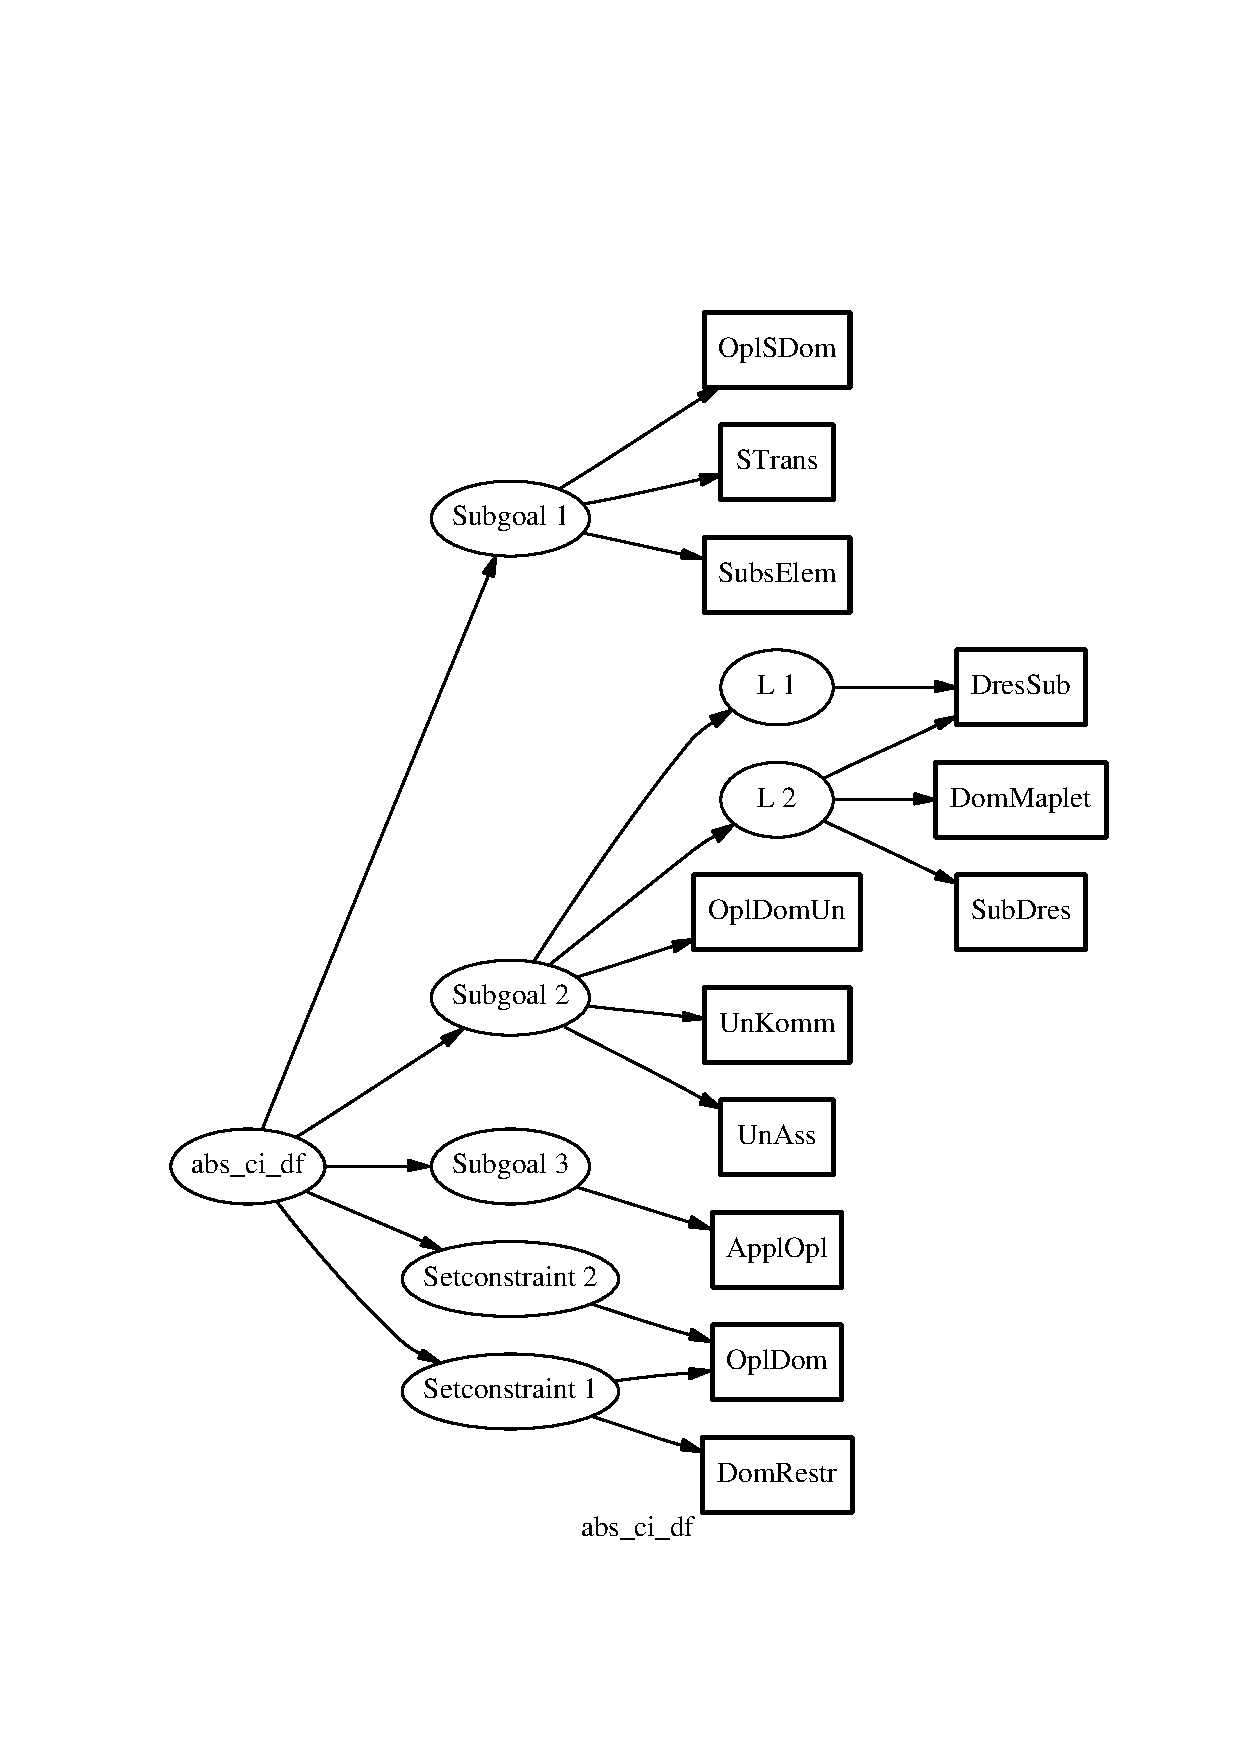
\includegraphics[]{pics/abs_ci_df_Graph_man.pdf}}}
\caption{A lemmagraph for the manual proof of $abs\_ci\_df$}%
\end{figure}%
%
%
%
\subsubsection{Computer Supported Proof}
%
% [Computer Supported Proof]
%
As mentioned at the beginning of this section, proofs of deadlock-free
consistency conditions can get arbitrarily hard to handle. To complete such a
task, we will see that it is profitable to use a mechanical proof. Although a
paper and pencil proof is essential, automatic simplification and management of
assumptions, side conditions (to name just a few examples) can significantly
reduce the required time and
increase trust in the stability of it.\\
The manual proof we have shown has been the basis for the computer supported
proof. The idea of having side conditions in a proof is realised implicitly by
the theorem prover. Completing the goal with the additional assumption
$rep'(abs\_cvsauth) \in \dom abs\_auth\_of$ is a mixture of redrawing the proof
shown before and using simplification routines and automatic tactics. Using and
improving a lemma library and gathering subtasks combining tacticals and
ML-functions leads to a
remarkably fast and short result.\\

Given a syntactic precondition, the goals can be generated uniformly using the HOL-Z-\LaTeX-style.\\[0.4cm]
%
% orginal (modified a little):
%
% (zcomment + naming)
%
\newsavebox{\sampleAbsCiDFBox}
\begin{lrbox}{\sampleAbsCiDFBox}
\begin{minipage}{.9\linewidth}
\ensuremath {abs\_ci\_df}\hfill \\
\zcomment{\begin {dzed}
abs\_ci\_df == 
[ClientState; RepositoryState; files? : \power Abs\_Name | (wfiles \cap files?) \subseteq \dom wc]
\implies \pre abs\_ci
\end{dzed}}
\end{minipage}
\end{lrbox}
\newcommand{\sampleAbsCiDF}{\usebox{\sampleAbsCiDFBox }}
%
% now, use it:
\sampleAbsCiDF\mbox{}\\[0.4cm]
%
%
%
To give an overview, we also add the lemmagraph of the Isabelle proof.
Sometimes, we needed slightly different instances of the lemmas used in the
manual proof. The machine supported proof has been constructed top down. At
first, the main lemmas were proven. Then the main proof was built
linking the lemmas by backward reasoning. Some steps mentioned in
the manual proof were proven automatically.
% 
% 
\begin{figure}%
\rotatebox{0}{\scalebox{0.8}{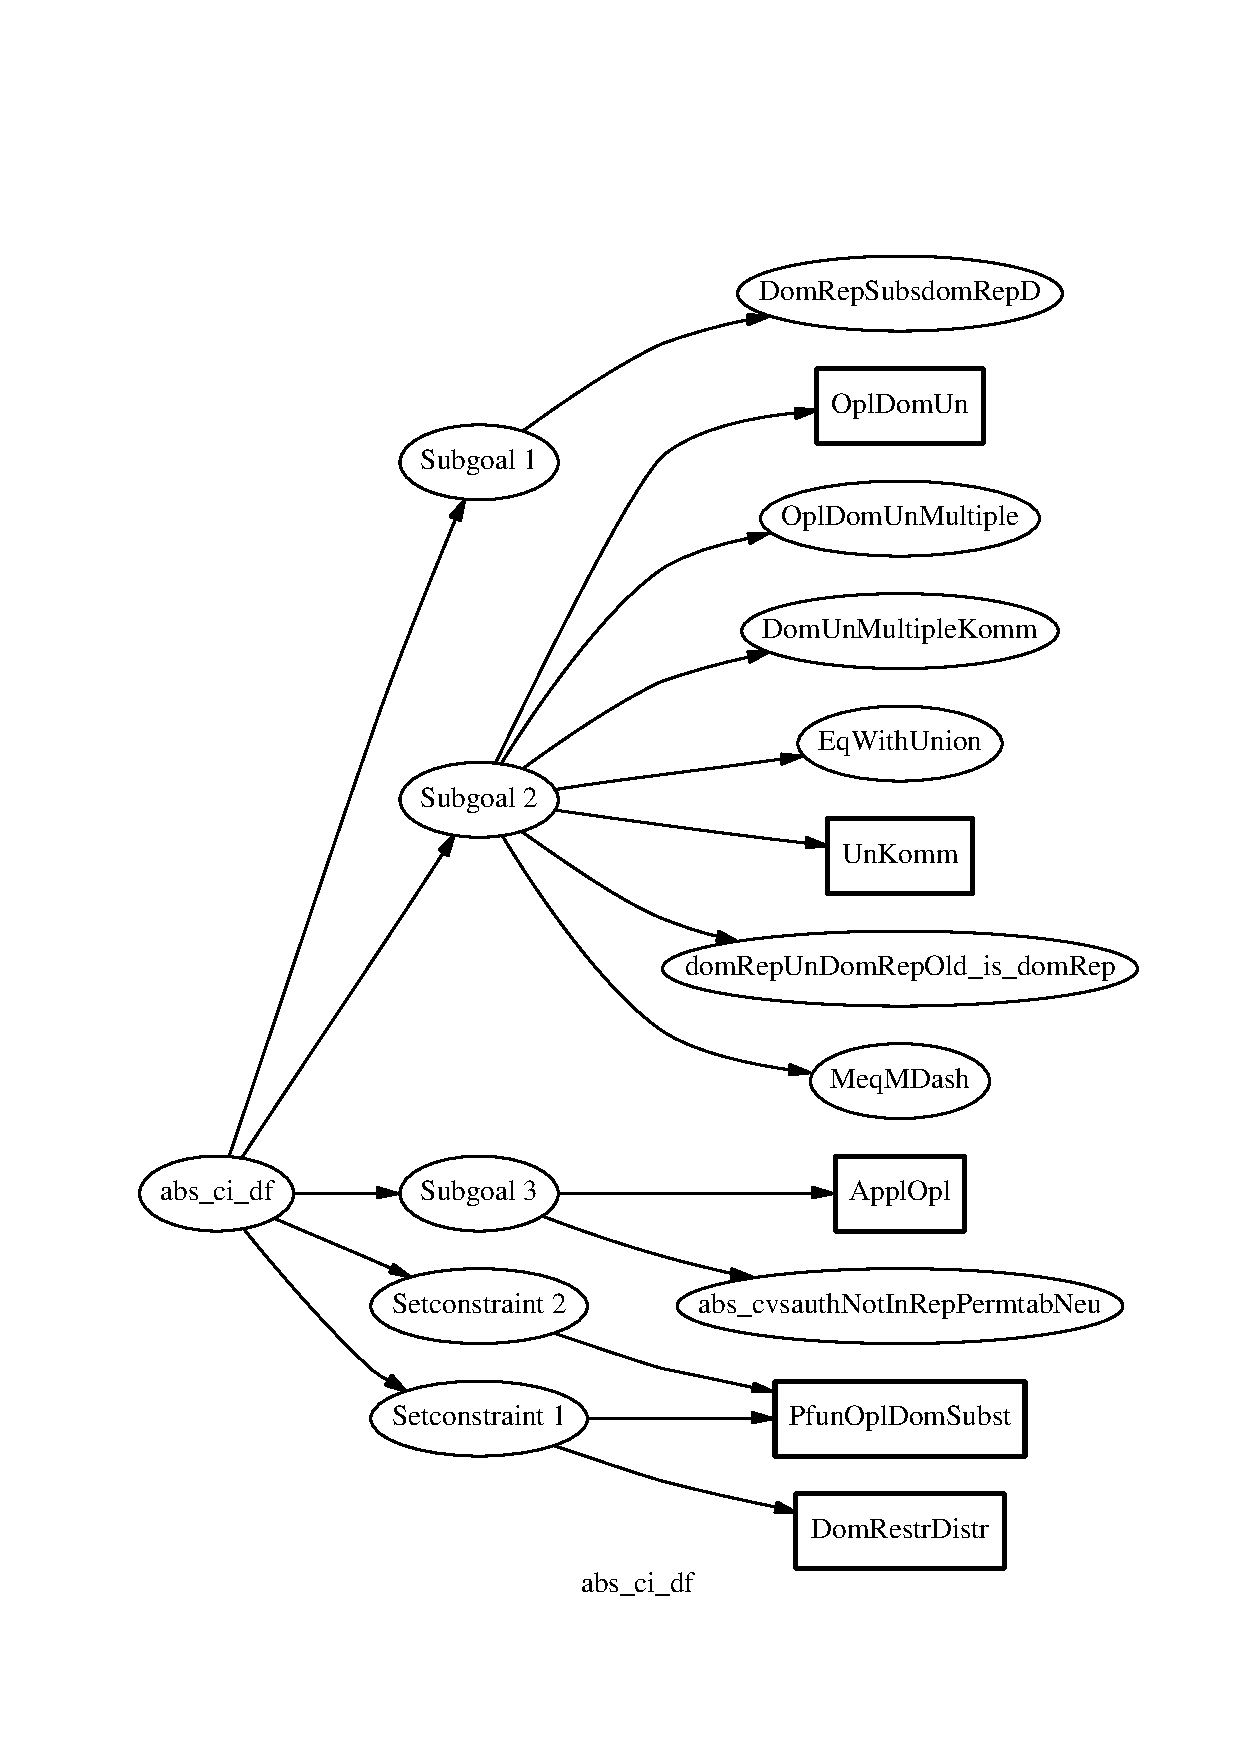
\includegraphics[]{pics/abs_ci_df_Graph.pdf}}}
\caption{A lemmagraph for the proof of $abs\_ci\_df$ using Isabelle/HOL-Z}%
\end{figure}%
%
%
% 
%
\newpage

\section{Verifying the Refinement}
\label{sec:refinement}

\zsection[AbsOperations,CVSServer]{Refinement}\vspace{1ex}\noindent

In this section, we focus on the refinement of the data types of our abstract
system architecture to data structures of our concrete implementation
architecture.  In particular, we will map the CVS repository and working copy to
a \unix file system and permissions to file attributes.

In order to prove that the concrete data structures correctly implements the
abstract data types, we have to define an abstraction schema $R$ which relates
the components of the abstract state schemas to the components of the concrete
implementation state schemas and thereby explains which concrete states
represent which abstract states.

The definition of this relating schema needs auxiliary functions $Rdata$ and
$Rname2path$ that map abstract data to concrete data, i.e.\ files, and the
abstract names of files to paths in the \unix file system.  Since we are not
concerned about the content of the files (except the administration files of
CVS), a very rough specification of these functions suffices.
\begin{axdef}
  Rdata: Abs\_Data \bij Data \\
  Rname2path: Abs\_Name \bij Path \\
  \where
% FRANK: was soll das?
%  \forall p: \ran Rname2path @ cvs\_rep \prefix p \\
  Rname2path(abs\_cvsauth) = cvs\_rep \cat \langle CVSROOT, cvsauth \rangle \\
\end{axdef}

Now we can proceed to define the abstraction schema $R$.  Importing the abstract
and concrete state schemas introduces all components that have to be set into
relation.  Note that some components ($cvs\_uid$ or $passwd$ for example) of the
abstract state also appear in the concrete state.  These components have the
same meaning in both states and do not need to be related in this schema.  The
set $wfiles$ of names of the abstract state, which is used to control the access
operations, must be related to the concrete working directory $wdir$.
Furthermore, we require that the files in the working copy $wc$ and in the
repository $rep$ of the abstract state have corresponding files in the
appropriate directories of the concrete file system $files$.  We also require
that the permission tables in the abstract and in the concrete state are the
same and that the roles and passwords that are assigned to each file in the
working copy of the abstract state have corresponding attributes in the concrete
state.
\begin{schema}{R}
  ClientState \\
  RepositoryState \\
  ProcessState \\
  Cvs\_FileSystem \\
  \where
  abs\_passwd = cvs\_passwd \\

  \forall n: wfiles @ wdir \prefix Rname2path(n) \\
  
  Rname2path \limg \dom wc \rimg = \dom wcs\_attributes \\

  authtab(rep) = get\_auth\_tab(files) \\
  \forall n: \dom rep @ \exists f: \dom files@ cvs\_rep \prefix f \\
  \t1 \land Rname2path(n) = f \land Inl(Rdata(rep~n)) = files(f) \\
  \forall n: \dom wc @ wc\_uidtab(n) = ((wcs\_attributes(Rname2path~n)).f\_uid)  \\
  \forall n: \dom wc @ \exists f: \dom files @ \lnot (cvs\_rep \prefix f) \\
  \forall f: \dom rep @ \exists ps: \power Perm | \{ru,rg\} \subseteq ps @ \\
  \t1 attributes(Rname2path~f) = \lbind \< perm == ps, \\
  uid == cvsperm2uid(rep\_permtab~f), \\
  gid == cvsperm2gid(rep\_permtab~f) \rbind \>
\end{schema}

Closely following the refinement notion of Spivey~\cite{spivey:z_notation:1992},
we must prove two refinement conditions for each operation on the abstract state
$\sigma_{abs}$ and its corresponding operation on the concrete state
$\sigma_{conc}$.  However, the original setting assumes that the abstract
operation $op_{abs}$ and the corresponding concrete operation $op_{conc}$ are
defined over the same input and output parameters, which does not always hold
for our operations.  Therefore, we extend the original refinement notion by
(sometimes) strengthening the premises of the refinement conditions.

\paragraph{Refinement condition (I1)}
A concrete operation $op_{conc}$ can make a transition whenever its
corresponding abstract operation $op_{abs}$ can make a transition (i.e.\ a
successor state $\sigma'_{conc}$ exists). The situation is depicted in
Figure~\ref{fig:refcon1}.
\begin{figure}[h!]
    \center
      \scalebox{0.5}{\input{pics/ref_concept1}}
    \caption{Refinement Condition (I1).\label{fig:refcon1}}
\end{figure}

In other words, condition (I1) ensures that a concrete operation terminates
whenever its corresponding abstract operation is guaranteed to terminate. For
input parameters $in?$, this is formalized as:
\zcomment{
  \begin{zed}
    \forall \sigma_{abs}; \sigma_{conc}; in?: T_1 @ \pre op_{abs} \land R
    \implies \pre op_{conc} \\ 
  \end{zed}}


\paragraph{Refinement condition (I2)}
For any possible state $\sigma'_{conc}$ reachable by the concrete operation,
there must be a $R$-related state $\sigma'_{abs}$ that can be reached by the
abstract operation, provided that the initial states $\sigma_{abs}$ and
$\sigma_{conc}$ had been $R$-related. The situation is depicted in
Figure~\ref{fig:refcon2}.
\begin{figure}[h!]
    \center
      \scalebox{0.5}{\input{pics/ref_concept2}}
    \caption{Refinement Condition (I2).\label{fig:refcon2}}
\end{figure}

This condition ensures that the state after the concrete operation represents
one of those abstract states in which the abstract operation could terminate.
For input parameters $in?$ and output parameters $out!$, this is represented
formally:
\zcomment{
  \begin{zed}
    \forall \sigma_{abs}; \sigma_{conc}; \sigma'_{conc}; in?: T_1; out!: T_2
    @ \\
    \t1 \pre op_{abs} \land R \land op_{conc} \implies (\exists
    \sigma'_{abs} @ R' \land op_{abs}) \\
  \end{zed}}
  
Additionally, there is the requirement that the initial states are compatible:
\paragraph{Refinement condition (II)}
Each possible initial state of the concrete type must represent a possible
initial state of the abstract type.
\zcomment{
  \begin{zed}
    \forall \sigma_{conc} @ Init_{conc} \implies (\exists \sigma_{abs} @
    Init_{abs} \land R) \\
  \end{zed}}

In the following subsections, we will list the proof obligations for the
refinement in full detail. The proofs can be found in the in the HOL-Z
distribution (see \verb+examples/zeta/cvs-server/holz+). The proofs are highly
non-trivial.

%\subsection{Examples of Refinement}

%\subsubsection{Refinement of the initial states}
%The initialization schemas for the abstract and concrete state are
%missing.\fixme{FRANK: Initialzustaende fehlen noch!}

\subsection{The login operation}
As a first simple example, we show the two conditions (I1) and (I2) for the CVS
\cvscmd{login} command, which is used to initially authenticate a client to the
CVS server.  For the definition of the operation schemas, we refer to the
$abs\_login$ schema in the abstract section, and the $cvs\_login$ schema in the
implementation section.

We need the additional preconditions that the requested role and the supplied
passwords are the same on the abstract and concrete level. Here, we
intentionally did not give the input parameters the same names since this leads
to problems in the generated refinement proof-obligations; the standard
refinement notion implicitly requires abstract and concrete states to have
distinct bindings. Since we cannot use arbitrary formulas in schema calculus
expressions, we must wrap a schema $Asm\_login$ around these preconditions:
\begin{schema}{Asm\_login}
  passwd?, cvs\_pwd?: Cvs\_Passwd \\   
  uid?, cvs\_uid?: Cvs\_Uid \\
  \where
  passwd? = cvs\_pwd? \land uid? = cvs\_uid? \\
\end{schema}


\begin{schema}{pre\_of\_cvs\_login}
  files: FILESYS\_TAB \\
  cvs\_uid?: Cvs\_Uid \\
  cvs\_pwd?: Cvs\_Passwd \\
  \where
  (cvs\_uid?,cvs\_pwd?) \in \dom(get\_auth\_tab~files) \\
\end{schema}
\begin{schema}{pre\_of\_abs\_login}
  uid?: Cvs\_Uid \\
  passwd?: Cvs\_Passwd \\
  rep: ABS\_DATATAB \\
  \where
  (uid?,passwd?) \in \dom(authtab~rep) \\
\end{schema}

\begin{axdef}
  PreLogin: \nat \\
  \where
  \forall Cvs\_FileSystem; ProcessState; Cvs\_FileSystem '; ProcessState '; \\
  \t1 cvs\_uid?: Cvs\_Uid; cvs\_pwd?: Cvs\_Passwd @ \\
  \t2 pre\_of\_cvs\_login \implies \pre cvs\_login \\

  \forall ClientState; RepositoryState; ClientState '; RepositoryState '; \\
  \t1 uid?: Cvs\_Uid; passwd?: Cvs\_Passwd @
  pre\_of\_abs\_login \implies \pre abs\_login \\
\end{axdef}

%%adb
\zrefinesOp[Astate={ClientState,RepositoryState},
            Cstate={ProcessState,Cvs\string\_FileSystem},
            Aop=abs\string\_login,
            Cop=cvs\string\_login,
            Args={passwd?: Cvs\string\_Passwd, cvs\string\_pwd?:
            Cvs\string\_Passwd, uid?: Cvs\string\_Uid, cvs\string\_uid?: 
            Cvs\string\_Uid}, 
            Abs=R,
            Assumption=Asm\string\_login,
            display
            ]{login}


\subsection{The add operation}

\begin{schema}{Asm\_add}
  p?: Path \\
  newfiles?: ABS\_DATATAB \\
  wdir: Path \\
  \where
  \forall n: \dom newfiles? @ wdir \cat p? \prefix Rname2path(n) \\
\end{schema}

\zrefinesOp[Astate={ClientState,RepositoryState},
            Cstate={ProcessState,Cvs\string\_FileSystem},
            Aop=abs\string\_add,
            Cop=cvs\string\_add,
            Args={newfiles?: ABS\string\_DATATAB; p?: Path},
            Abs=R,
            Assumption=Asm\string\_add,
            display
            ]{add}



\subsection{The update operation}

\begin{schema}{Asm\_update}
  p?: Path \\
  files?: \power Abs\_Name \\
  wdir: Path \\
  \where
  \forall n: files? @ wdir \cat p? \prefix Rname2path(n) \\
\end{schema}


\begin{schema}{pre\_of\_cvsUp}
  p?: Path \\
  files: FILESYS\_TAB \\
  wcs\_attributes: CVS\_ATTR\_TAB \\
  wdir: Path \\
  uid: Uid \\
  attributes: FILEATTR\_TAB \\
  \where
  cvs\_rep \cat repOf(wcs\_attributes~wdir) \cat p? \in \dom files \\
  has\_w\_access(uid, wdir \cat p?, attributes) \\
\end{schema}
\begin{schema}{pre\_of\_cvsUpErr}
  p?: Path \\
  wdir: Path \\
  uid: Uid \\
  attributes: FILEATTR\_TAB \\
  \where
  \lnot (has\_w\_access(uid, wdir \cat p?, attributes)) \\
\end{schema}
\begin{schema}{pre\_of\_cvsUpNoAct}
  p?: Path \\
  files: FILESYS\_TAB \\
  wcs\_attributes: CVS\_ATTR\_TAB \\
  wdir: Path \\
  uid: Uid \\
  attributes: FILEATTR\_TAB \\
  \where
  cvs\_rep \cat repOf(wcs\_attributes~wdir) \cat p? \notin \dom files \\
\end{schema}
\begin{axdef}
  PreUpdate: \nat \\
  \where
  \forall Cvs\_FileSystem; ProcessState; Cvs\_FileSystem '; ProcessState '; \\
  \t1 p?: Path; files: FILESYS\_TAB; wcs\_attributes: CVS\_ATTR\_TAB; \\
  \t1 wdir: Path; uid: Uid; attributes: FILEATTR\_TAB; error!: \denotation @ \\
  \t2 pre\_of\_cvsUp \implies \pre cvsUp \\

  \forall Cvs\_FileSystem; ProcessState; Cvs\_FileSystem '; ProcessState '; \\
  \t1 p?: Path; files: FILESYS\_TAB; wcs\_attributes: CVS\_ATTR\_TAB; \\
  \t1 wdir: Path; uid: Uid; attributes: FILEATTR\_TAB; error!: \denotation @ \\
  \t2 pre\_of\_cvsUpNoAct \implies \pre cvsUpNoAct \\

  \forall Cvs\_FileSystem; ProcessState; Cvs\_FileSystem '; ProcessState '; \\
  \t1 p?: Path; files: FILESYS\_TAB; wcs\_attributes: CVS\_ATTR\_TAB; \\
  \t1 wdir: Path; uid: Uid; attributes: FILEATTR\_TAB; error!: \denotation @ \\
  \t2 pre\_of\_cvsUpErr \implies \pre cvsUpErr \\
\end{axdef}

\zrefinesOp[Astate={ClientState,RepositoryState},
            Cstate={ProcessState,Cvs\string\_FileSystem},
            Aop=abs\string\_up,
            Cop=cvs\string\_update,
            Args={p?: Path; files?: \string\power\space Abs\string\_Name},
            Abs=R,
            Assumption=Asm\string\_update,
            display
            ]{update}

\subsection{The commit operation}

The schema $Asm\_ci$ defines the assumption that the current user has read
access to the working directory.  This must be stated in a separate assumption
because the abstract state has no notion of read/write/execute rights on files.
\begin{schema}{Asm\_ci}
  uid: Uid \\
  wdir: Path \\
  attributes: FILEATTR\_TAB \\
  p?: Path \\
  files?: \power Abs\_Name \\
  \where
  has\_r\_access(uid, wdir \cat p?, attributes) \\
  \forall n: files? @ wdir \cat p? \prefix Rname2path(n) \\
\end{schema}
\noindent With the assumptions in $Asm\_ci$ we can now formulate the refinement
proof obligations for the commit operations:

\zrefinesOp[Astate={ClientState,RepositoryState},
            Cstate={ProcessState,Cvs\string\_FileSystem},
            Aop=abs\string\_ci,
            Cop=cvs\string\_ci,
            Args={p?: Path; files?: \string\power\space Abs\string\_Name},
            Abs=R,
            Assumption=Asm\string\_ci,
            display
            ]{ci}

\subsection{The cd operation}

To relate the parameters of the abstract and the concrete $cd$ operation, we
define the schema $Asm\_cd$.  We require that all abstract files, which are to
be focused ($wfiles?$) must be related to a concrete file within the current
working directory $wdir$ (appended by some path $p?$) or one of its
subdirectories.

Setting the focus to a set of files in the abstract model corresponds to setting
the working directory (which also represents a set of files, namely all files
within it or within one of its subdirectories).
\begin{schema}{Asm\_cd}
  wfiles?: \power Abs\_Name \\
  p?, wdir: Path \\
  \where
  \forall n: wfiles? @ wdir \cat p? \prefix Rname2path(n) \\
\end{schema}
\noindent For this operation it suffices to only take $FileSystem$ into account,
not $Cvs\_Filesystem$.

\zrefinesOp[Astate={ClientState,RepositoryState},
            Cstate={ProcessState,FileSystem},
            Aop=abs\string\_cd,
            Cop=cd,
            Args={p?: Path; wfiles?: \string\power\space Abs\string\_Name},
            Abs=R,
            Assumption=Asm\string\_cd,
            display
            ]{cd}




%%% Local Variables:
%%% TeX-master: "arch"
%%% fill-column:80
%%% x-symbol-8bits:nil
%%% End:

% LocalWords:  conservativity conjoints
